\chapter{Ejemplos RMI}

Para compilar los ejemplos tenemos que:

\begin{itemize}
	\item Tener un archivo \texttt{server.policy}
	\item Haber ejecutado \texttt{rmiregistry} en una terminal, como es un proceso
	bloqueante se puede añadir el símborlo \& para ejecutarlo en segundo plano
	\item Compilar los ficheros \texttt{.java} con \texttt{javac}.
	\item Usar la siguiente orden seguida del nombre del fichero para ejecutar desde donde este el fichero \texttt{server.policy}:
	\begin{lstlisting}[language=sh]
		java -cp . -Djava.rmi.server.codebase=file:./ -Djava.rmi.server.hostname=localhost -Djava.security.policy=server.policy "fichero a ejecutar"
	\end{lstlisting}
\end{itemize}

\section{Ejemplo 1}
En este ejemplo se envía un mensaje simple desde el cliente para invocar al servidor. Despues de compilar lo ejecutaríamos así:
\begin{lstlisting}[language=sh]
	java -cp . -Djava.rmi.server.codebase=file:./ -Djava.rmi.server.hostname=localhost -Djava.security.policy=server.policy ejemplo1.Ejemplo
	java -cp . -Djava.rmi.server.codebase=file:./ -Djava.rmi.server.hostname=localhost -Djava.security.policy=server.policy ejemplo1.Cliente_Ejemplo localhost 1554
\end{lstlisting}

El número que añadimos al cliente es la hebra que va a invocar al objeto remoto del servidos, cada una de las órdenes anteriores debe estar en una terminal.

\begin{figure}[!ht]
	\begin{center}
		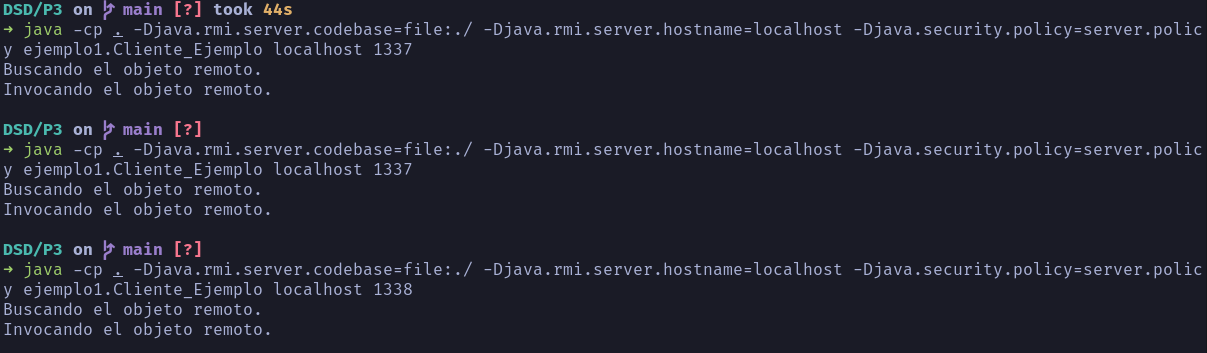
\includegraphics[scale=0.5]{clienteEjemplo1.png}
	\end{center}
\end{figure}

\begin{figure}[!ht]
	\begin{center}
		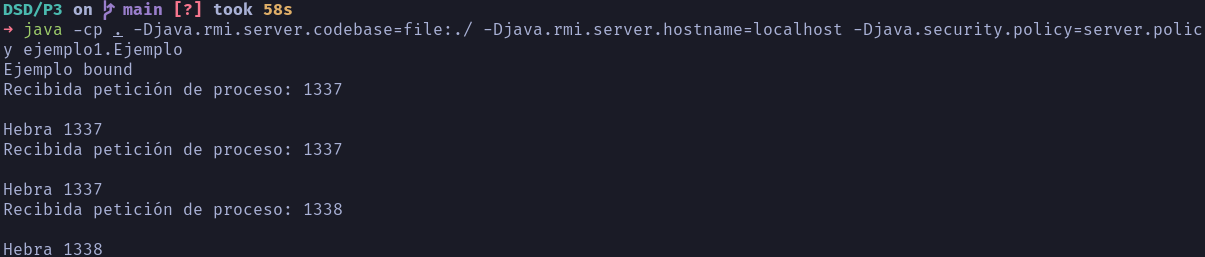
\includegraphics[scale=0.5]{servidorEjemplo1.png}
	\end{center}
\end{figure}

Si además el número fuese 0 el servidor ``dormiría'' durante 5 segundos:

\begin{figure}[!ht]
	\begin{center}
		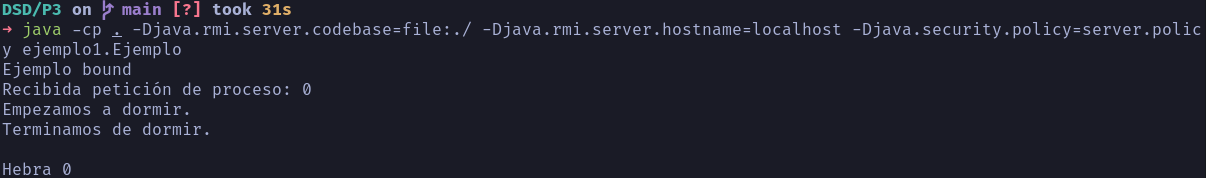
\includegraphics[scale=0.5]{servidorDormido.png}
	\end{center}
\end{figure}
\begin{figure}[!ht]
	\begin{center}
		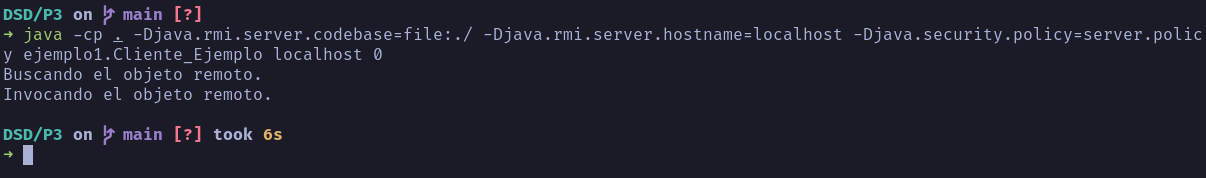
\includegraphics[scale=0.5]{cliente0.png}
	\end{center}
\end{figure}

\section{Ejemplo 2}

Este ejemplo es parecido al anterior, solo que en este caso desde el cliente se especifica
un número de hebras que llamarán al objeto remoto del servidor.

Para ejecutarlo usamos:

\begin{lstlisting}[language=sh]
	java -cp . -Djava.rmi.server.codebase=file:./ -Djava.rmi.server.hostname=localhost -Djava.security.policy=server.policy ejemplo2.Ejemplo
	java -cp . -Djava.rmi.server.codebase=file:./ -Djava.rmi.server.hostname=localhost -Djava.security.policy=server.policy ejemplo2.Cliente_Ejemplo_Multi_Thread localhost 5
\end{lstlisting}

Y el resultado es el siguiente:

\begin{figure}[!ht]
	\begin{center}
		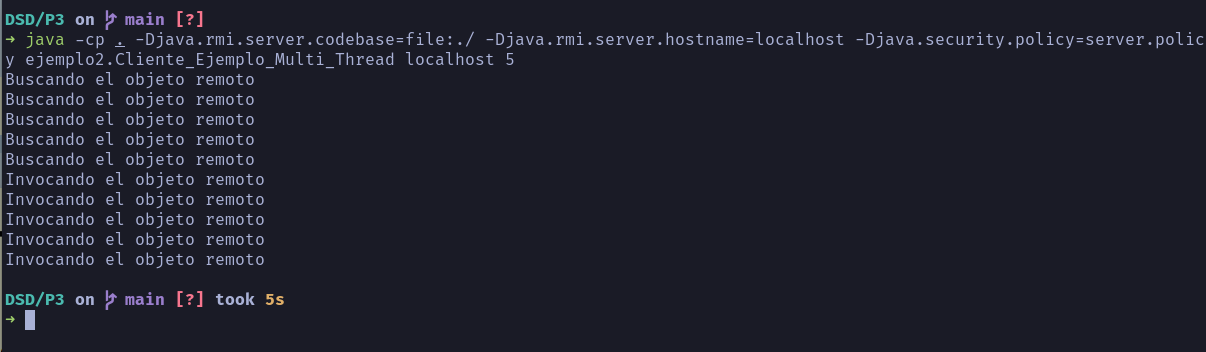
\includegraphics[scale=0.5]{clienteEjemplo2.png}
	\end{center}
\end{figure}

\begin{figure}[!ht]
	\begin{center}
		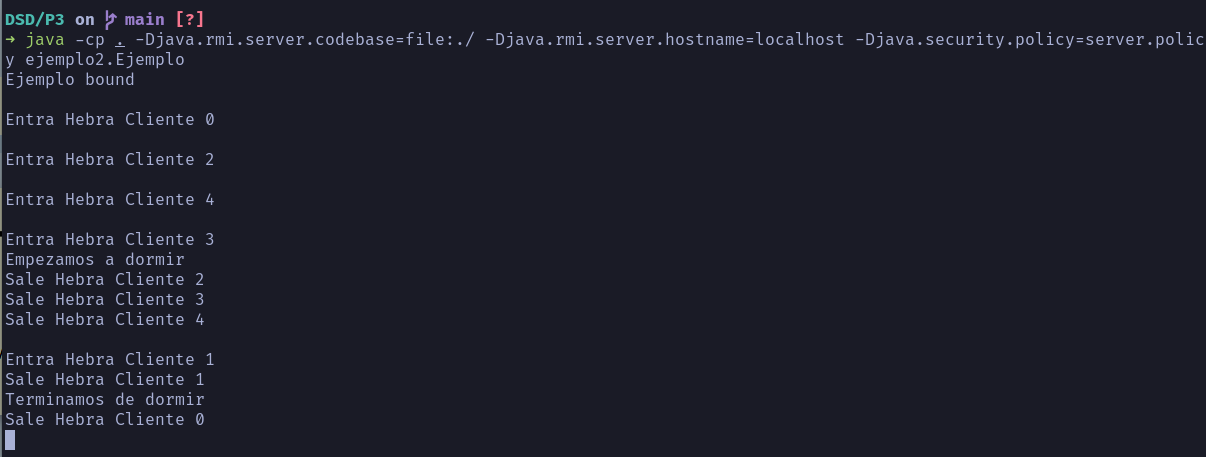
\includegraphics[scale=0.5]{servidorEjemplo2.png}
	\end{center}
\end{figure}

\section{Ejemplo 3}

Ejecutamos el cliente y servidor con las siguientes órdenes:

\begin{lstlisting}[language=sh]
	java -cp . -Djava.rmi.server.codebase=file:./ -Djava.rmi.server.hostname=localhost -Djava.security.policy=server.policy ejemplo3.Servidor
	java -cp . -Djava.rmi.server.codebase=file:./ -Djava.rmi.server.hostname=localhost -Djava.security.policy=server.policy ejemplo3.Cliente
\end{lstlisting}

En este ejemplo se llama varias veces a un objeto remoto \texttt{Contador} desde su interfaz \texttt{Contador\_I}
incrementando un valor local y devuelve el tiempo que ha tardado como resultado de hacer las peticiones indicadas en el código.

\begin{figure}[!ht]
	\begin{center}
		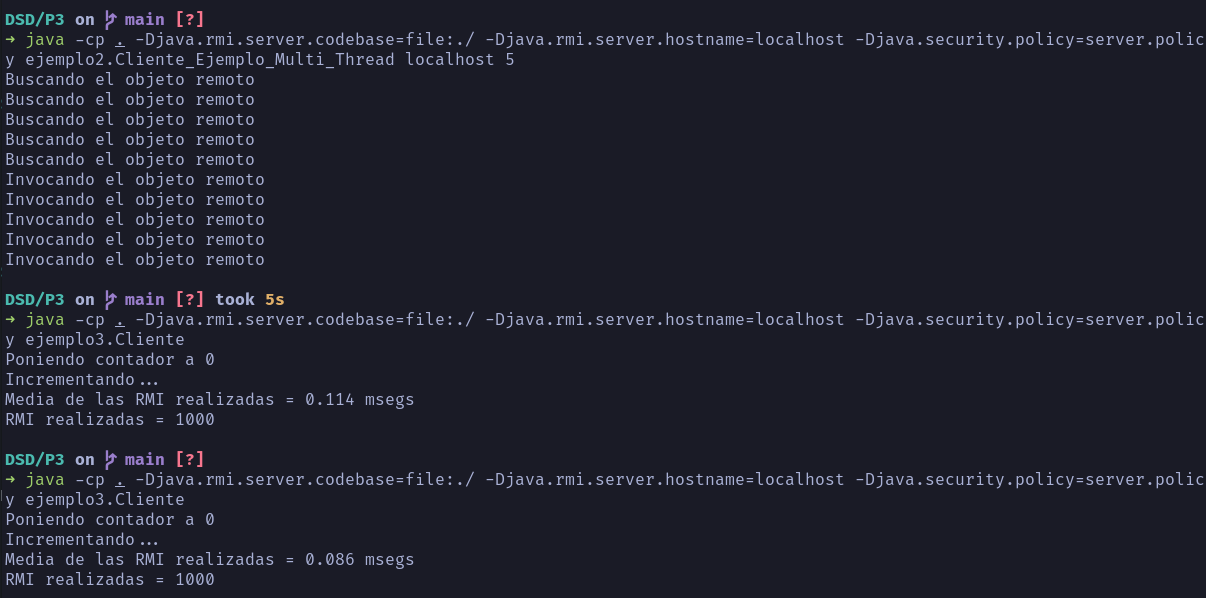
\includegraphics[scale=0.5]{ejemplo3.png}
	\end{center}
\end{figure}
